\documentclass[10 pt]{beamer}
\usetheme{Madrid}
\usepackage[utf8]{inputenc}
\usepackage{default}
\usepackage{xspace}
\usepackage{graphicx,graphics} 
\usepackage{color}
\usepackage{amsmath}
\usepackage{amsfonts}
\usepackage{amssymb}
\usepackage{amsthm}
\usepackage{algorithm}
\usepackage{algorithmic}
\usepackage{longtable}
\usepackage{complexity}
\usepackage{tkz-graph}
\usepackage{float}
\usepackage{setspace}

\tikzset{
  LabelStyle/.style = { rectangle, rounded corners, draw,
                       font = \bfseries },
  EdgeStyle/.append style = {-} }
\title{Contention management for Deterministic Networking}

\author{Maël~Guiraud}


\institute[Nokia Bell Labs, DAVID-UVSQ] 
{
  DAVID, Universit\'e de Versailles Saint Quentin -
  Nokia Bell Labs France \\
}

\subject{Theoretical Computer Science}

\begin{document}

\begin{frame}

  \titlepage
  \centering
  \includegraphics [width=15mm]{logod.png} \hspace{1cm} \includegraphics [width=20mm]{logon.png} \hspace{1cm} \includegraphics [width=20mm]{logo.png} \\
\end{frame}

\begin{frame}

  \tableofcontents[]
\end{frame}


\begin{section}{Presentation}

\begin{frame}{Context}
  \centering
  \includegraphics[scale=0.2]{bts.png}\\
  A base transceiver station.

\end{frame}


\begin{frame}{Context}
  \centering
  \includegraphics[scale=0.2]{cloudbts.png}\\
  \includegraphics[scale=0.175]{BBURRH.png}
\end{frame}


% \begin{frame}{Context}
%   \centering
%   \includegraphics[scale=0.38]{fronthaul.png}
% \end{frame}


\begin{frame}{Model}
\begin{center}
 


\scalebox{0.5}{
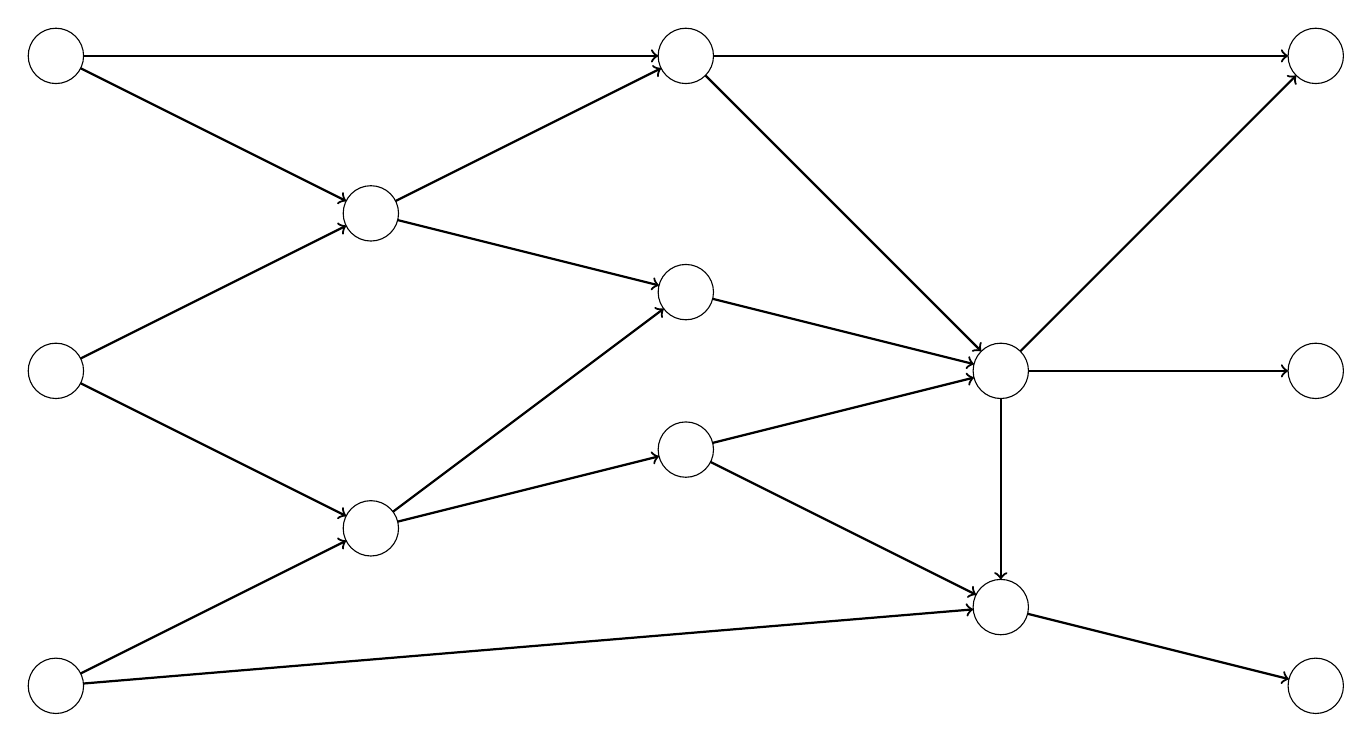
\begin{tikzpicture}
  \SetGraphUnit{5}
    \tikzset{
  EdgeStyle/.append style = {->} }
   \tikzstyle{VertexStyle}=[shape = circle, draw, minimum size = 20pt]
    \SetVertexNoLabel
  \Vertex[x=0,y=0]{a3}
  \Vertex[x=0,y=4]{a2}
  \Vertex[x=0,y=8]{a1}
  
  
  \Vertex[x=16,y=0]{c3}
  \Vertex[x=16,y=4]{c2}
  \Vertex[x=16,y=8]{c1}
  

  \Vertex[x=4,y=2]{n1}
  \Vertex[x=4,y=6]{n2}  
  \Vertex[x=12,y=1]{n3}
  \Vertex[x=12,y=4]{n4}
  \Vertex[x=8,y=3]{n6}
  \Vertex[x=8,y=5]{n7}
  \Vertex[x=8,y=8]{n8}

  \Edge(a1)(n2)
  \Edge(a1)(n8)
  \Edge(a2)(n2)
  \Edge(a2)(n1)
  \Edge(a3)(n1)
  \Edge(a3)(n3)
  \Edge(n8)(n4)
  \Edge(n8)(c1)
  \Edge(n2)(n8)
  \Edge(n2)(n7)
  \Edge(n1)(n7)
  \Edge(n1)(n6)
  \Edge(n6)(n3)
  \Edge(n6)(n4)
  \Edge(n7)(n4)
  \Edge(n4)(c1)
  \Edge(n4)(c2)
  \Edge(n4)(n3)
  \Edge(n3)(c3)

\end{tikzpicture}
}

 Network $\rightarrow$ Graph $G=(V,A)$.\\


 \end{center}
\end{frame}


\begin{frame}{Model}
\begin{center}
 


\scalebox{0.5}{
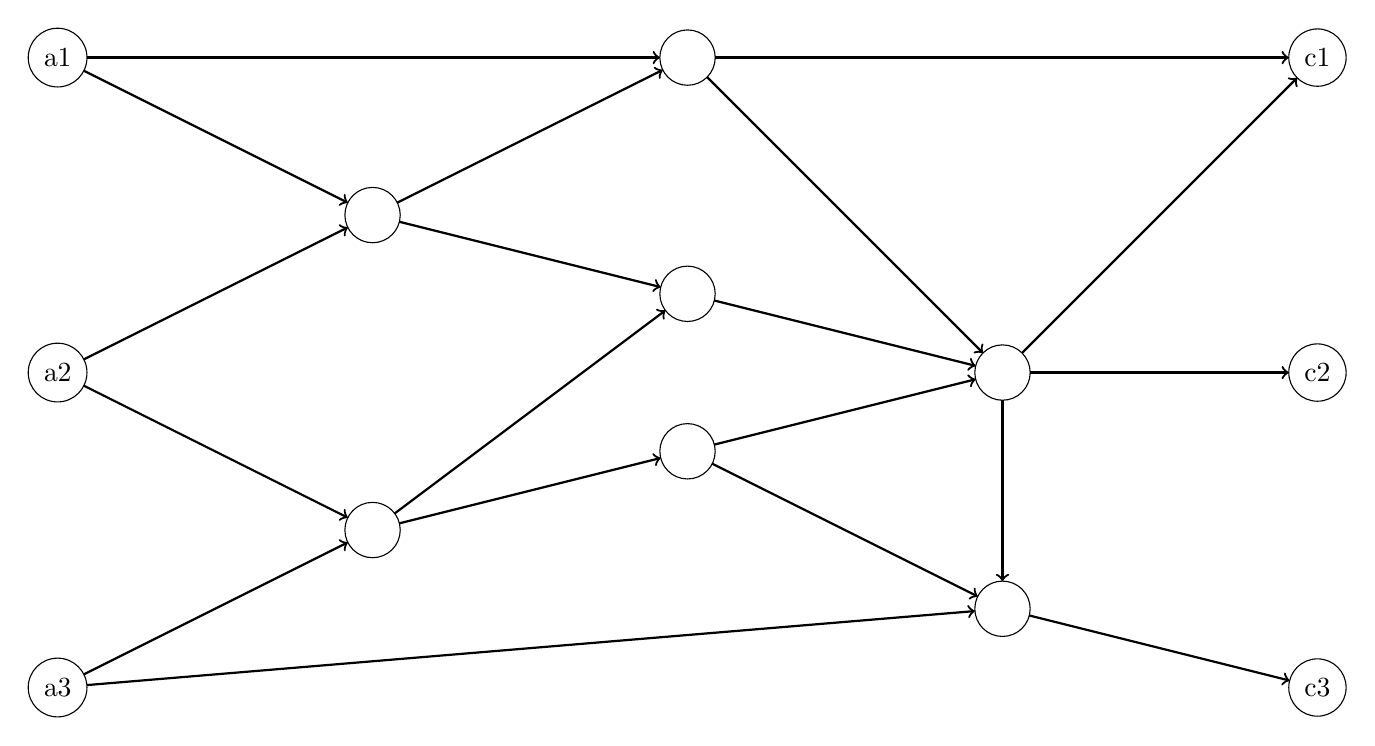
\begin{tikzpicture}
  \SetGraphUnit{5}
    \tikzset{
  EdgeStyle/.append style = {->} }
   \tikzstyle{VertexStyle}=[shape = circle, draw, minimum size = 20pt]
  \Vertex[x=0,y=0]{a3}
  \Vertex[x=0,y=4]{a2}
  \Vertex[x=0,y=8]{a1}
  
  
  \Vertex[x=16,y=0]{c3}
  \Vertex[x=16,y=4]{c2}
  \Vertex[x=16,y=8]{c1}
  
 \SetVertexNoLabel
  \Vertex[x=4,y=2]{n1}
  \Vertex[x=4,y=6]{n2}  
  \Vertex[x=12,y=1]{n3}
  \Vertex[x=12,y=4]{n4}
  \Vertex[x=8,y=3]{n6}
  \Vertex[x=8,y=5]{n7}
  \Vertex[x=8,y=8]{n8}

  \Edge(a1)(n2)
  \Edge(a1)(n8)
  \Edge(a2)(n2)
  \Edge(a2)(n1)
  \Edge(a3)(n1)
  \Edge(a3)(n3)
  \Edge(n8)(n4)
  \Edge(n8)(c1)
  \Edge(n2)(n8)
  \Edge(n2)(n7)
  \Edge(n1)(n7)
  \Edge(n1)(n6)
  \Edge(n6)(n3)
  \Edge(n6)(n4)
  \Edge(n7)(n4)
  \Edge(n4)(c1)
  \Edge(n4)(c2)
  \Edge(n4)(n3)
  \Edge(n3)(c3)

\end{tikzpicture}
}


 RRH / BBU $\rightarrow$ set of vertices A (Antennas) and C (Computation).\\


 \end{center}
\end{frame}

\begin{frame}{Model}
\begin{center}
 


\scalebox{0.5}{
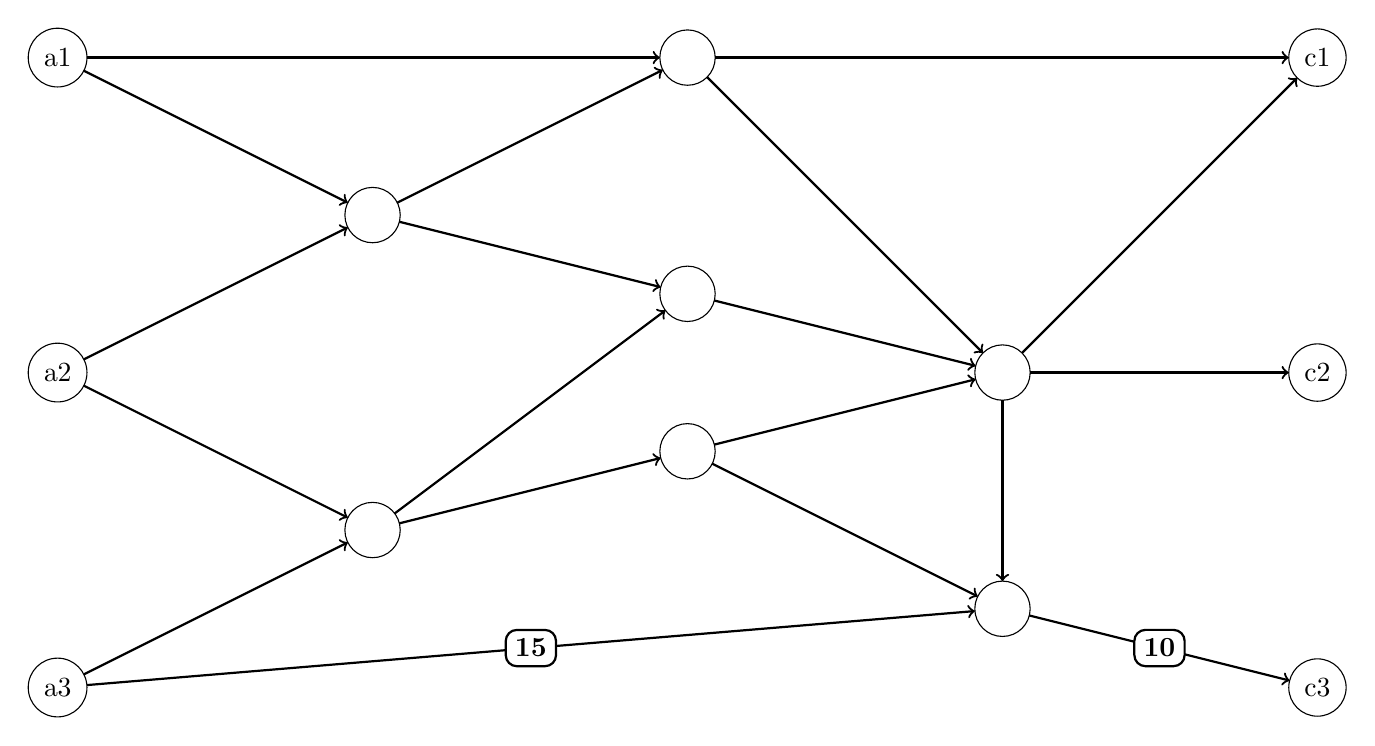
\begin{tikzpicture}
  \SetGraphUnit{5}
    \tikzset{
  EdgeStyle/.append style = {->} }
   \tikzstyle{VertexStyle}=[shape = circle, draw, minimum size = 20pt]
  \Vertex[x=0,y=0]{a3}
  \Vertex[x=0,y=4]{a2}
  \Vertex[x=0,y=8]{a1}
  
  
  \Vertex[x=16,y=0]{c3}
  \Vertex[x=16,y=4]{c2}
  \Vertex[x=16,y=8]{c1}
  
 \SetVertexNoLabel
  \Vertex[x=4,y=2]{n1}
  \Vertex[x=4,y=6]{n2}  
  \Vertex[x=12,y=1]{n3}
  \Vertex[x=12,y=4]{n4}
  \Vertex[x=8,y=3]{n6}
  \Vertex[x=8,y=5]{n7}
  \Vertex[x=8,y=8]{n8}

  \Edge(a1)(n2)
  \Edge(a1)(n8)
  \Edge(a2)(n2)
  \Edge(a2)(n1)
  \Edge(a3)(n1)
  \Edge[label = 15](a3)(n3)
  \Edge(n8)(n4)
  \Edge(n8)(c1)
  \Edge(n2)(n8)
  \Edge(n2)(n7)
  \Edge(n1)(n7)
  \Edge(n1)(n6)
  \Edge(n6)(n3)
  \Edge(n6)(n4)
  \Edge(n7)(n4)
  \Edge(n4)(c1)
  \Edge(n4)(c2)
  \Edge(n4)(n3)
  \Edge[label = 10](n3)(c3)

\end{tikzpicture}
}


 Physical Delay of a link $\rightarrow$ Weight on arcs.\\


 \end{center}
\end{frame}


\begin{frame}{Model}
\begin{center}
 


\scalebox{0.5}{
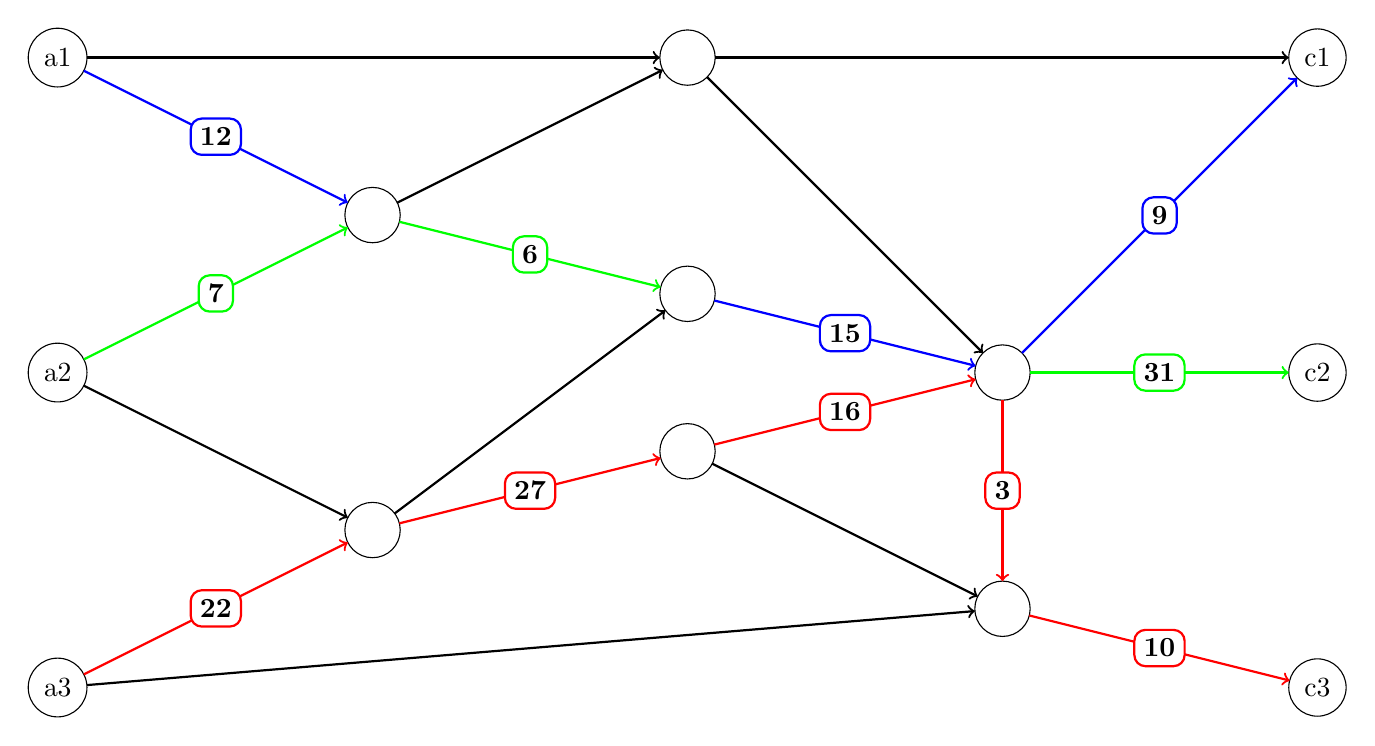
\begin{tikzpicture}
  \SetGraphUnit{5}
    \tikzset{
  EdgeStyle/.append style = {->} }
   \tikzstyle{VertexStyle}=[shape = circle, draw, minimum size = 20pt]
  \Vertex[x=0,y=0]{a3}
  \Vertex[x=0,y=4]{a2}
  \Vertex[x=0,y=8]{a1}
  
  
  \Vertex[x=16,y=0]{c3}
  \Vertex[x=16,y=4]{c2}
  \Vertex[x=16,y=8]{c1}
  
 \SetVertexNoLabel
  \Vertex[x=4,y=2]{n1}
  \Vertex[x=4,y=6]{n2}  
  \Vertex[x=12,y=1]{n3}
  \Vertex[x=12,y=4]{n4}
  \Vertex[x=8,y=3]{n6}
  \Vertex[x=8,y=5]{n7}
  \Vertex[x=8,y=8]{n8}


  \Edge(a1)(n8)
 
  \Edge(a2)(n1)

  \Edge(a3)(n3)
  \Edge(n8)(n4)
  \Edge(n8)(c1)
  \Edge(n2)(n8)

  \Edge(n1)(n7)

  \Edge(n6)(n3)
 
 

  
  \tikzset{
  EdgeStyle/.append style = {blue} }
  \Edge[label = 12](a1)(n2)
  \Edge[label = 9](n4)(c1)
   
      \Edge[label = 15](n7)(n4)

   \tikzset{
  EdgeStyle/.append style = {red} }
    \Edge[label = 22](a3)(n1)
   \Edge[label = 10](n3)(c3)
     \Edge[label = 27](n1)(n6)
    \Edge[label = 16](n6)(n4)
    \Edge[label = 3](n4)(n3)
       \tikzset{
  EdgeStyle/.append style = {green} }
   \Edge[label = 7](a2)(n2)
  \Edge[label = 31](n4)(c2)
  \Edge[label = 6](n2)(n7)



\end{tikzpicture}
}

Coherent routing.\\


 \end{center}

\end{frame}




\begin{frame}{Message sending}
 \begin{block}{Slotted time}
  A time (in slots) can be :
  \begin{itemize}
   \item A delay on a link.
   \item The time taken to emit a message.
  \end{itemize}
 \end{block}

  \begin{block}{Message sending}
  Reserving slots on a route.

\centering
\scalebox{0.3}{

\begin{tikzpicture}
  \SetGraphUnit{5}
    \tikzset{
  EdgeStyle/.append style = {->} }
   \tikzstyle{VertexStyle}=[shape = circle, draw, minimum size = 20pt]
  \Vertex[x=0,y=0]{a3}
  \Vertex[x=0,y=4]{a2}
  \Vertex[x=0,y=8]{a1}
  
  
  \Vertex[x=16,y=0]{c3}
  \Vertex[x=16,y=4]{c2}
  \Vertex[x=16,y=8]{c1}
  
 \SetVertexNoLabel
  \Vertex[x=4,y=2]{n1}
  \Vertex[x=4,y=6]{n2}  
  \Vertex[x=12,y=1]{n3}
  \Vertex[x=12,y=4]{n4}
  \Vertex[x=8,y=3]{n6}
  \Vertex[x=8,y=5]{n7}
  \Vertex[x=8,y=8]{n8}


  \Edge(a1)(n8)
 
  \Edge(a2)(n1)

  \Edge(a3)(n3)
  \Edge(n8)(n4)
  \Edge(n8)(c1)
  \Edge(n2)(n8)

  \Edge(n1)(n7)

  \Edge(n6)(n3)

  
  \tikzset{
  EdgeStyle/.append style = {blue} }
  \Edge(a1)(n2)
  \Edge(n4)(c1)
   
      \Edge(n7)(n4)

   \tikzset{
  EdgeStyle/.append style = {red} }
    \Edge(a3)(n1)
   \Edge(n3)(c3)
     \Edge(n1)(n6)
    \Edge(n6)(n4)
    \Edge(n4)(n3)
       \tikzset{
  EdgeStyle/.append style = {green} }
   \Edge(a2)(n2)
  \Edge(n4)(c2)
  \Edge(n2)(n7)
  \node (0) at (5,1.5){\includegraphics[scale=0.2]{chronogrames/4.jpeg}};
  \node (1) at (1,-1){\includegraphics[scale=0.2]{chronogrames/0.jpeg}};

\end{tikzpicture}
}
 \end{block}

\end{frame}


\begin{frame}{Collisions}
 
\centering
\scalebox{0.5}{

\begin{tikzpicture}
  \SetGraphUnit{5}
    \tikzset{
  EdgeStyle/.append style = {->} }
   \tikzstyle{VertexStyle}=[shape = circle, draw, minimum size = 20pt]
  \Vertex[x=0,y=0]{a3}
  \Vertex[x=0,y=4]{a2}
  \Vertex[x=0,y=8]{a1}
  
  
  \Vertex[x=16,y=0]{c3}
  \Vertex[x=16,y=4]{c2}
  \Vertex[x=16,y=8]{c1}
  
 \SetVertexNoLabel
  \Vertex[x=4,y=2]{n1}
  \Vertex[x=4,y=6]{n2}  
  \Vertex[x=12,y=1]{n3}
  \Vertex[x=12,y=4]{n4}
  \Vertex[x=8,y=3]{n6}
  \Vertex[x=8,y=5]{n7}
  \Vertex[x=8,y=8]{n8}


  \Edge(a1)(n8)
 
  \Edge(a2)(n1)

  \Edge(a3)(n3)
  \Edge(n8)(n4)
  \Edge(n8)(c1)
  \Edge(n2)(n8)

  \Edge(n1)(n7)

  \Edge(n6)(n3)
 
 

  
  \tikzset{
  EdgeStyle/.append style = {blue} }
  \Edge(a1)(n2)
  \Edge(n4)(c1)
   
      \Edge(n7)(n4)

   \tikzset{
  EdgeStyle/.append style = {red} }
    \Edge(a3)(n1)
   \Edge(n3)(c3)
     \Edge(n1)(n6)
    \Edge(n6)(n4)
    \Edge(n4)(n3)
       \tikzset{
  EdgeStyle/.append style = {green} }
   \Edge(a2)(n2)
  \Edge(n4)(c2)
  \Edge(n2)(n7)

  \node (0) at (14,3.5){\includegraphics[scale=0.2]{chronogrames/3.jpeg}};


\end{tikzpicture}
}

There is a collision when a slot is used by many routes.

\end{frame}

\begin{section}{Problem}

\begin{frame}{Problem}
 
\centering
\scalebox{0.5}{

\begin{tikzpicture}
  \SetGraphUnit{5}
    \tikzset{
  EdgeStyle/.append style = {->} }
   \tikzstyle{VertexStyle}=[shape = circle, draw, minimum size = 20pt]
  \Vertex[x=0,y=0]{a3}
  \Vertex[x=0,y=4]{a2}
  \Vertex[x=0,y=8]{a1}
  
  
  \Vertex[x=16,y=0]{c3}
  \Vertex[x=16,y=4]{c2}
  \Vertex[x=16,y=8]{c1}
  
 \SetVertexNoLabel
  \Vertex[x=4,y=2]{n1}
  \Vertex[x=4,y=6]{n2}  
  \Vertex[x=12,y=1]{n3}
  \Vertex[x=12,y=4]{n4}
  \Vertex[x=8,y=3]{n6}
  \Vertex[x=8,y=5]{n7}
  \Vertex[x=8,y=8]{n8}


  \Edge(a1)(n8)
 
  \Edge(a2)(n1)

  \Edge(a3)(n3)
  \Edge(n8)(n4)
  \Edge(n8)(c1)
  \Edge(n2)(n8)

  \Edge(n1)(n7)

  \Edge(n6)(n3)
 
 

  
  \tikzset{
  EdgeStyle/.append style = {blue} }
  \Edge(a1)(n2)
  \Edge(n4)(c1)
   
      \Edge(n7)(n4)

   \tikzset{
  EdgeStyle/.append style = {red} }
    \Edge(a3)(n1)
   \Edge(n3)(c3)
     \Edge(n1)(n6)
    \Edge(n6)(n4)
    \Edge(n4)(n3)
       \tikzset{
  EdgeStyle/.append style = {green} }
   \Edge(a2)(n2)
  \Edge(n4)(c2)
  \Edge(n2)(n7)

  
  \node (4) at (0,-1){\includegraphics[scale=0.05]{chronogrames/9.jpeg}};

  \node (5) at (0,3){\includegraphics[scale=0.05]{chronogrames/9.jpeg}};

  \node (6) at (0,7){\includegraphics[scale=0.05]{chronogrames/9.jpeg}};
  \node (3) at (14,3.5){\includegraphics[scale=0.2]{chronogrames/6.jpeg}};
  \node (2) at (0,7){\LARGE ?};
\node (0) at (0,-1){\LARGE ?};
  \node (1) at (0,3){\LARGE ?};
\end{tikzpicture}
}

The problem is to find the good starting time for each route such that there is no collision, considering a periodic process.

\end{frame}


\begin{frame}{NP-Hardness}
\begin{center}
 
 
\scalebox{0.35}{

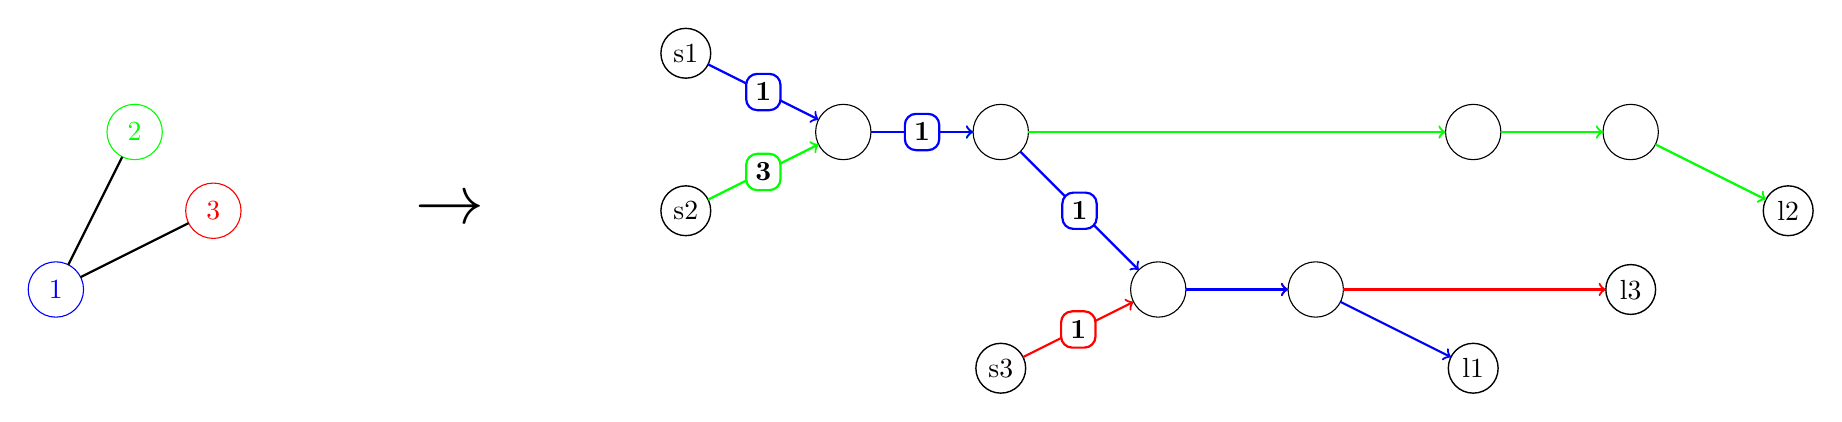
\begin{tikzpicture}

\tikzset{
  LabelStyle/.style = { rectangle, rounded corners, draw,
                       font = \bfseries },
  EdgeStyle/.append style = {->} }
  \SetGraphUnit{5}
  \Vertex[x=4,y=2]{s3}
  \Vertex[x=0,y=4]{s2}
  \Vertex[x=0,y=6]{s1}
  
  \Vertex[x=12,y=3]{l3}
  \Vertex[x=14,y=4]{l2}
  \Vertex[x=10,y=2]{l1}
  \tikzstyle{VertexStyle}=[shape = circle, draw, minimum size = 20pt]
     \tikzset{
  VertexStyle/.append style = {blue} }
    \Vertex[x=-8,y=3]{1}
          \tikzset{
  VertexStyle/.append style = {green} }
      \Vertex[x=-7,y=5]{2}

        \tikzset{
  VertexStyle/.append style = {red} }
      \Vertex[x=-6,y=4]{3}
             \tikzset{
  VertexStyle/.append style = {black} }
  
  
  \SetVertexNoLabel
  \Vertex[x=2,y=5]{A}
  \Vertex[x=4,y=5]{B}
  \Vertex[x=10,y=5]{C}
  \Vertex[x=12,y=5]{D}
  \Vertex[x=6,y=3]{E}
  \Vertex[x=8,y=3]{F}
  \tikzset{
  EdgeStyle/.append style = {green} }
  \Edge[label = 3](s2)(A)
  \Edge(A)(B)
  \Edge(B)(C)
  \Edge(C)(D)
  \Edge(D)(l2)

  
   \tikzset{
  EdgeStyle/.append style = {red} }
  \Edge[label = 1](s3)(E)
  \Edge(E)(F)
  \Edge(F)(l3) 
     \tikzset{
  EdgeStyle/.append style = {blue} }
  \Edge[label = 1](s1)(A)
  \Edge[label = 1](A)(B)
  \Edge[label = 1](B)(E)
  \Edge(E)(F)
  \Edge(F)(l1)
  
    \tikzset{
  EdgeStyle/.append style = {black,-} }

  \Edge(1)(2)
  \Edge(1)(3)
\node (1) at (-3,4){\Huge $\rightarrow$};
\end{tikzpicture}


}\\
\vspace{2cm}
 Reducing an instance of k-coloring into an instance of our problem.
 
 \end{center}
 \end{frame}


 

\begin{frame}{NP-Hardness}
\begin{center}
 
 
\scalebox{0.35}{

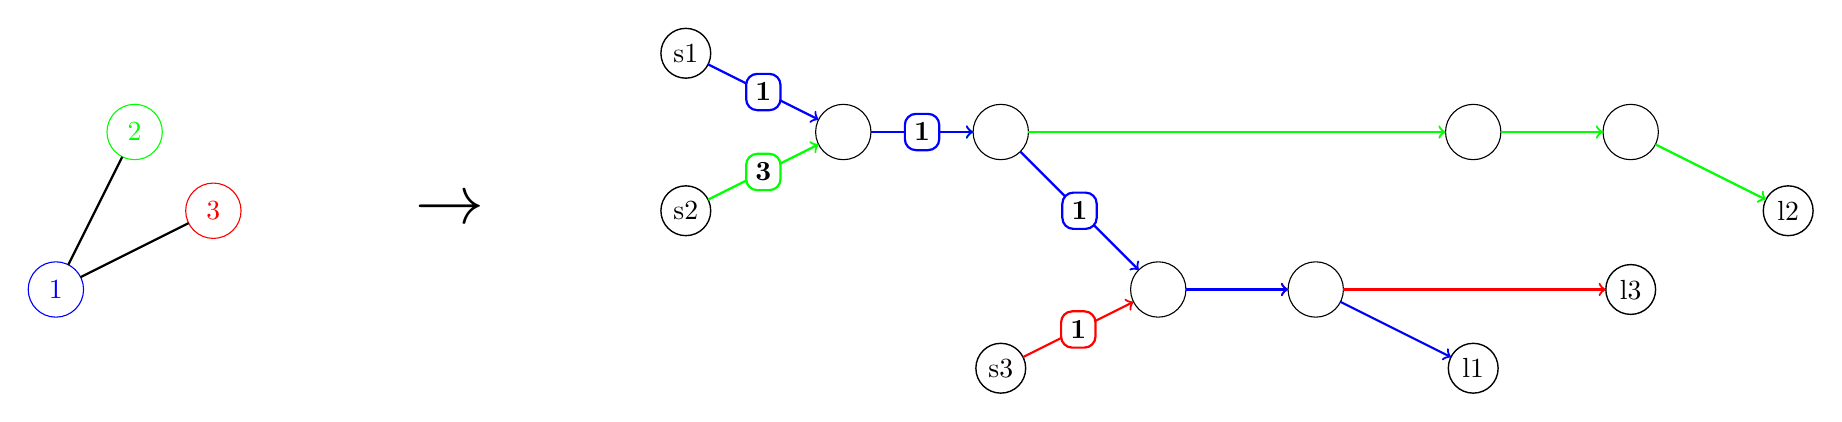
\begin{tikzpicture}

\tikzset{
  LabelStyle/.style = { rectangle, rounded corners, draw,
                       font = \bfseries },
  EdgeStyle/.append style = {->} }
  \SetGraphUnit{5}
  \Vertex[x=4,y=2]{s3}
  \Vertex[x=0,y=4]{s2}
  \Vertex[x=0,y=6]{s1}
  
  \Vertex[x=12,y=3]{l3}
  \Vertex[x=14,y=4]{l2}
  \Vertex[x=10,y=2]{l1}
  \tikzstyle{VertexStyle}=[shape = circle, draw, minimum size = 20pt]
     \tikzset{
  VertexStyle/.append style = {blue} }
    \Vertex[x=-8,y=3]{1}
          \tikzset{
  VertexStyle/.append style = {green} }
      \Vertex[x=-7,y=5]{2}

        \tikzset{
  VertexStyle/.append style = {red} }
      \Vertex[x=-6,y=4]{3}
             \tikzset{
  VertexStyle/.append style = {black} }
  
  
  \SetVertexNoLabel
  \Vertex[x=2,y=5]{A}
  \Vertex[x=4,y=5]{B}
  \Vertex[x=10,y=5]{C}
  \Vertex[x=12,y=5]{D}
  \Vertex[x=6,y=3]{E}
  \Vertex[x=8,y=3]{F}
  \tikzset{
  EdgeStyle/.append style = {green} }
  \Edge[label = 3](s2)(A)
  \Edge(A)(B)
  \Edge(B)(C)
  \Edge(C)(D)
  \Edge(D)(l2)

  
   \tikzset{
  EdgeStyle/.append style = {red} }
  \Edge[label = 1](s3)(E)
  \Edge(E)(F)
  \Edge(F)(l3) 
     \tikzset{
  EdgeStyle/.append style = {blue} }
  \Edge[label = 1](s1)(A)
  \Edge[label = 1](A)(B)
  \Edge[label = 1](B)(E)
  \Edge(E)(F)
  \Edge(F)(l1)
  
    \tikzset{
  EdgeStyle/.append style = {black,-} }

  \Edge(1)(2)
  \Edge(1)(3)
\node (1) at (-3,4){\Huge $\rightarrow$};
\end{tikzpicture}


}\\
\vspace{2cm}
 Give to the route 1 the offset(color) 0, and the route 2 and 3 the offset(color) 1.
 
 There is a 2 periodic affectation of the graph.
 \end{center}
 \end{frame}


\begin{frame}{Conflict Graph}
\begin{center}


 \begin{block}{Conflict graph}
   A conflict graph, is a digraph in which:
   \begin{itemize}
    \item The vertices are the route of the network.
    \item There is an edge between two vertices if the two routes have a common path.
    \item The weight on the edges is the difference between the conflict point and the sources of the routes.
   \end{itemize}

 \end{block}
 
\scalebox{0.35}{


 
 
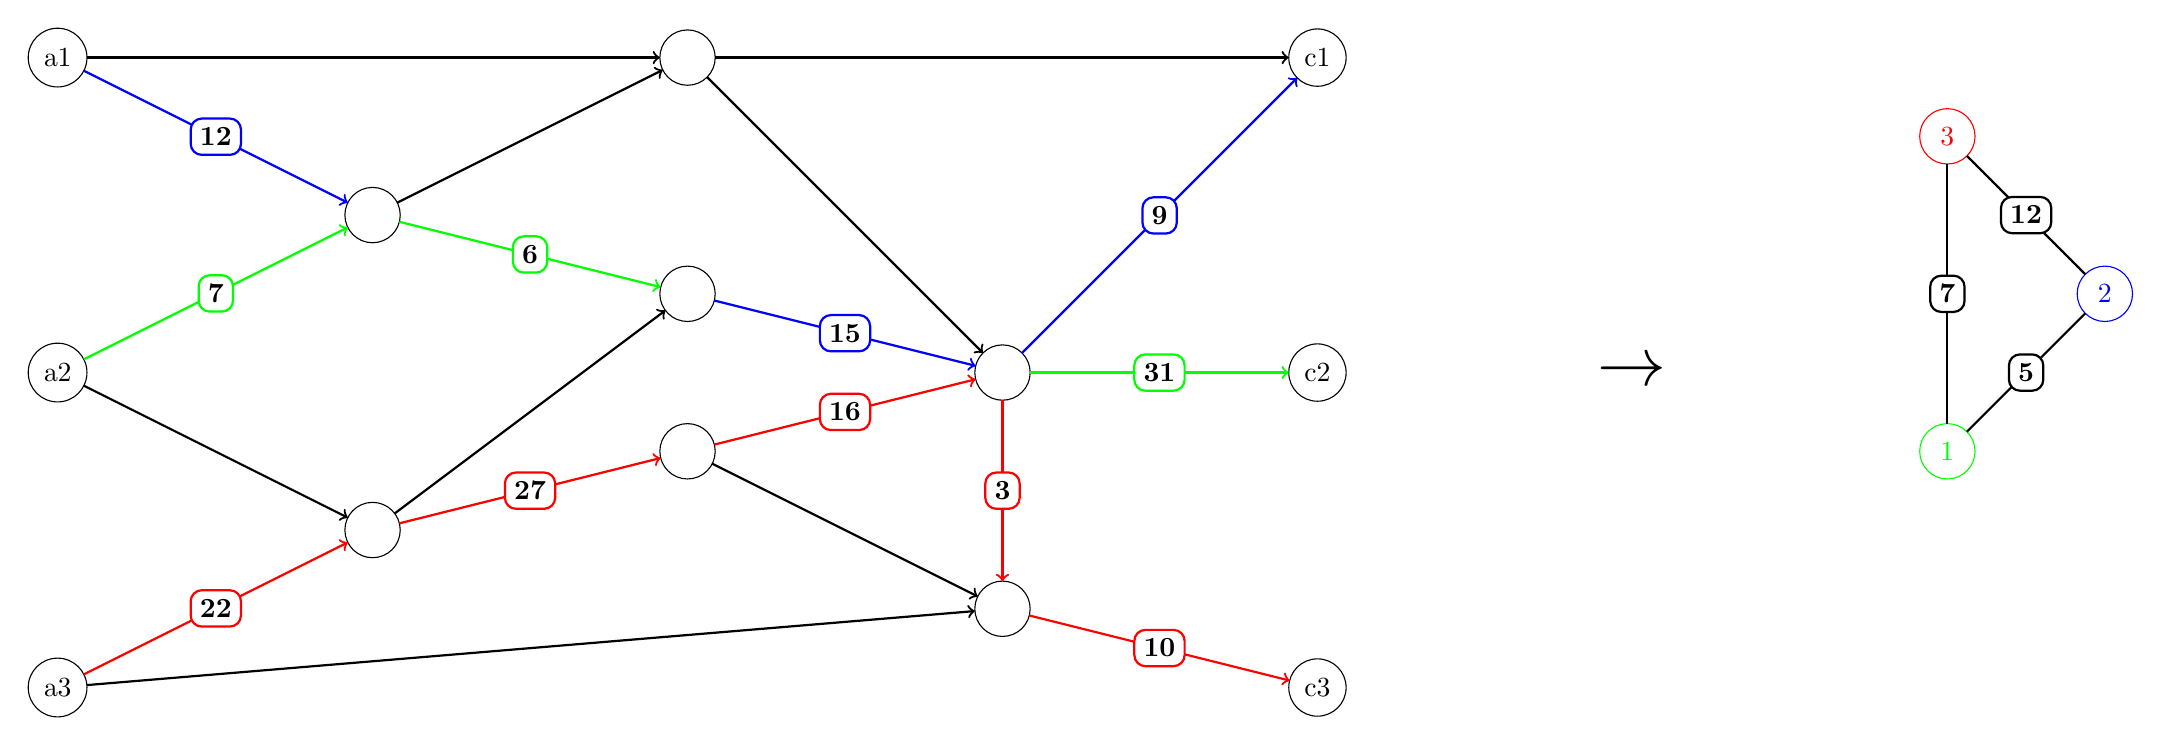
\begin{tikzpicture}
  \SetGraphUnit{5}
    \tikzset{
  EdgeStyle/.append style = {->} }
   \tikzstyle{VertexStyle}=[shape = circle, draw, minimum size = 20pt]
  \Vertex[x=0,y=0]{a3}
  \Vertex[x=0,y=4]{a2}
  \Vertex[x=0,y=8]{a1}


  
  
  \Vertex[x=16,y=0]{c3}
  \Vertex[x=16,y=4]{c2}
  \Vertex[x=16,y=8]{c1}

      \tikzset{
  VertexStyle/.append style = {blue} }
    \Vertex[x=26,y=5]{2}
          \tikzset{
  VertexStyle/.append style = {green} }
      \Vertex[x=24,y=3]{1}

        \tikzset{
  VertexStyle/.append style = {red} }
      \Vertex[x=24,y=7]{3}
             \tikzset{
  VertexStyle/.append style = {black} }
   \SetVertexNoLabel
  \Vertex[x=4,y=2]{n1}
  \Vertex[x=4,y=6]{n2}  
  \Vertex[x=12,y=1]{n3}
  \Vertex[x=12,y=4]{n4}
  \Vertex[x=8,y=3]{n6}
  \Vertex[x=8,y=5]{n7}
  \Vertex[x=8,y=8]{n8}


  \Edge(a1)(n8)
 
  \Edge(a2)(n1)

  \Edge(a3)(n3)
  \Edge(n8)(n4)
  \Edge(n8)(c1)
  \Edge(n2)(n8)

  \Edge(n1)(n7)

  \Edge(n6)(n3)
 
 

  
  \tikzset{
  EdgeStyle/.append style = {blue} }
  \Edge[label = 12](a1)(n2)
  \Edge[label = 9](n4)(c1)
   
      \Edge[label = 15](n7)(n4)

   \tikzset{
  EdgeStyle/.append style = {red} }
    \Edge[label = 22](a3)(n1)
   \Edge[label = 10](n3)(c3)
     \Edge[label = 27](n1)(n6)
    \Edge[label = 16](n6)(n4)
    \Edge[label = 3](n4)(n3)
       \tikzset{
  EdgeStyle/.append style = {green} }
   \Edge[label = 7](a2)(n2)
  \Edge[label = 31](n4)(c2)
  \Edge[label = 6](n2)(n7)


  
    \tikzset{
  EdgeStyle/.append style = {black,-} }


    \Edge[label = 7](1)(3)
    \Edge[label = 12](2)(3)
    \Edge[label = 5](2)(1)

    \node (1) at (20,4){\Huge $\rightarrow$};
  
\end{tikzpicture}
}
 \end{center}

\end{frame}

 
 
\begin{frame}{Conflict Graph}
\begin{center}
 

\scalebox{0.35}{


 
 
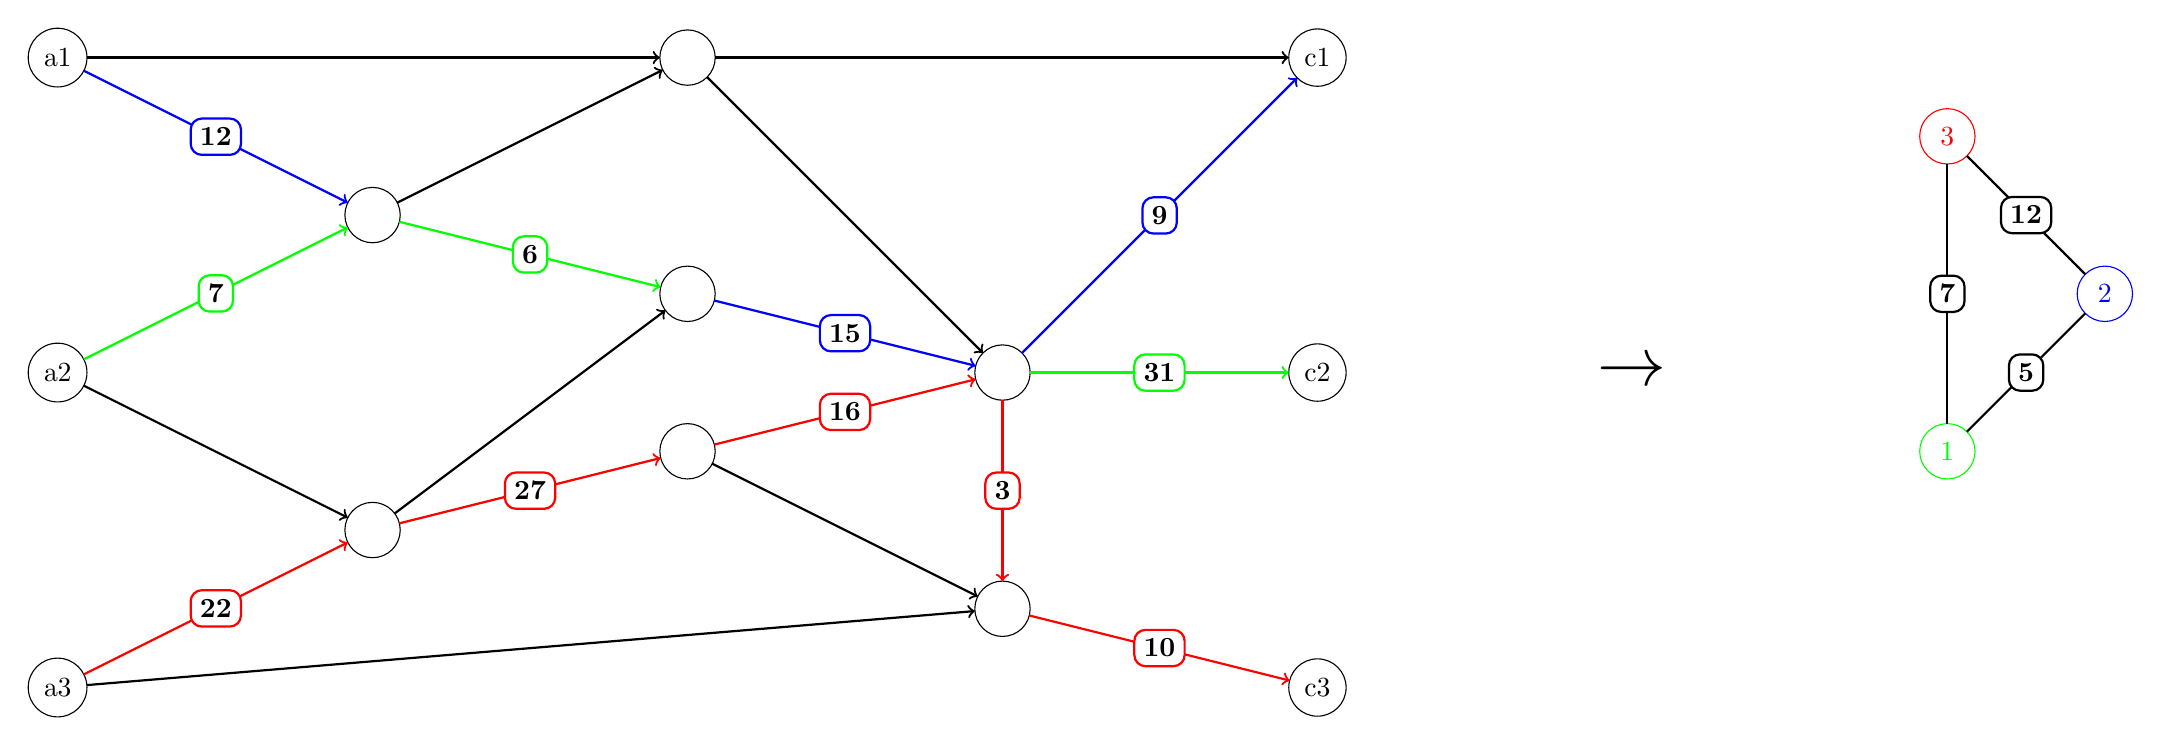
\begin{tikzpicture}
  \SetGraphUnit{5}
    \tikzset{
  EdgeStyle/.append style = {->} }
   \tikzstyle{VertexStyle}=[shape = circle, draw, minimum size = 20pt]
  \Vertex[x=0,y=0]{a3}
  \Vertex[x=0,y=4]{a2}
  \Vertex[x=0,y=8]{a1}


  
  
  \Vertex[x=16,y=0]{c3}
  \Vertex[x=16,y=4]{c2}
  \Vertex[x=16,y=8]{c1}

      \tikzset{
  VertexStyle/.append style = {blue} }
    \Vertex[x=26,y=5]{2}
          \tikzset{
  VertexStyle/.append style = {green} }
      \Vertex[x=24,y=3]{1}

        \tikzset{
  VertexStyle/.append style = {red} }
      \Vertex[x=24,y=7]{3}
             \tikzset{
  VertexStyle/.append style = {black} }
   \SetVertexNoLabel
  \Vertex[x=4,y=2]{n1}
  \Vertex[x=4,y=6]{n2}  
  \Vertex[x=12,y=1]{n3}
  \Vertex[x=12,y=4]{n4}
  \Vertex[x=8,y=3]{n6}
  \Vertex[x=8,y=5]{n7}
  \Vertex[x=8,y=8]{n8}


  \Edge(a1)(n8)
 
  \Edge(a2)(n1)

  \Edge(a3)(n3)
  \Edge(n8)(n4)
  \Edge(n8)(c1)
  \Edge(n2)(n8)

  \Edge(n1)(n7)

  \Edge(n6)(n3)
 
 

  
  \tikzset{
  EdgeStyle/.append style = {blue} }
  \Edge[label = 12](a1)(n2)
  \Edge[label = 9](n4)(c1)
   
      \Edge[label = 15](n7)(n4)

   \tikzset{
  EdgeStyle/.append style = {red} }
    \Edge[label = 22](a3)(n1)
   \Edge[label = 10](n3)(c3)
     \Edge[label = 27](n1)(n6)
    \Edge[label = 16](n6)(n4)
    \Edge[label = 3](n4)(n3)
       \tikzset{
  EdgeStyle/.append style = {green} }
   \Edge[label = 7](a2)(n2)
  \Edge[label = 31](n4)(c2)
  \Edge[label = 6](n2)(n7)


  
    \tikzset{
  EdgeStyle/.append style = {black,-} }


    \Edge[label = 7](1)(3)
    \Edge[label = 12](2)(3)
    \Edge[label = 5](2)(1)
  \node (1) at (20,4){\Huge $\rightarrow$};
  
  
\end{tikzpicture}
}

Labelling the conflict graph $\rightarrow$ finding a scheduling for the graph G.

 \end{center}

\end{frame}
\end{section}


\begin{section}{Application}


\begin{frame}{General Problem}
  \centering
  
\scalebox{0.5}{
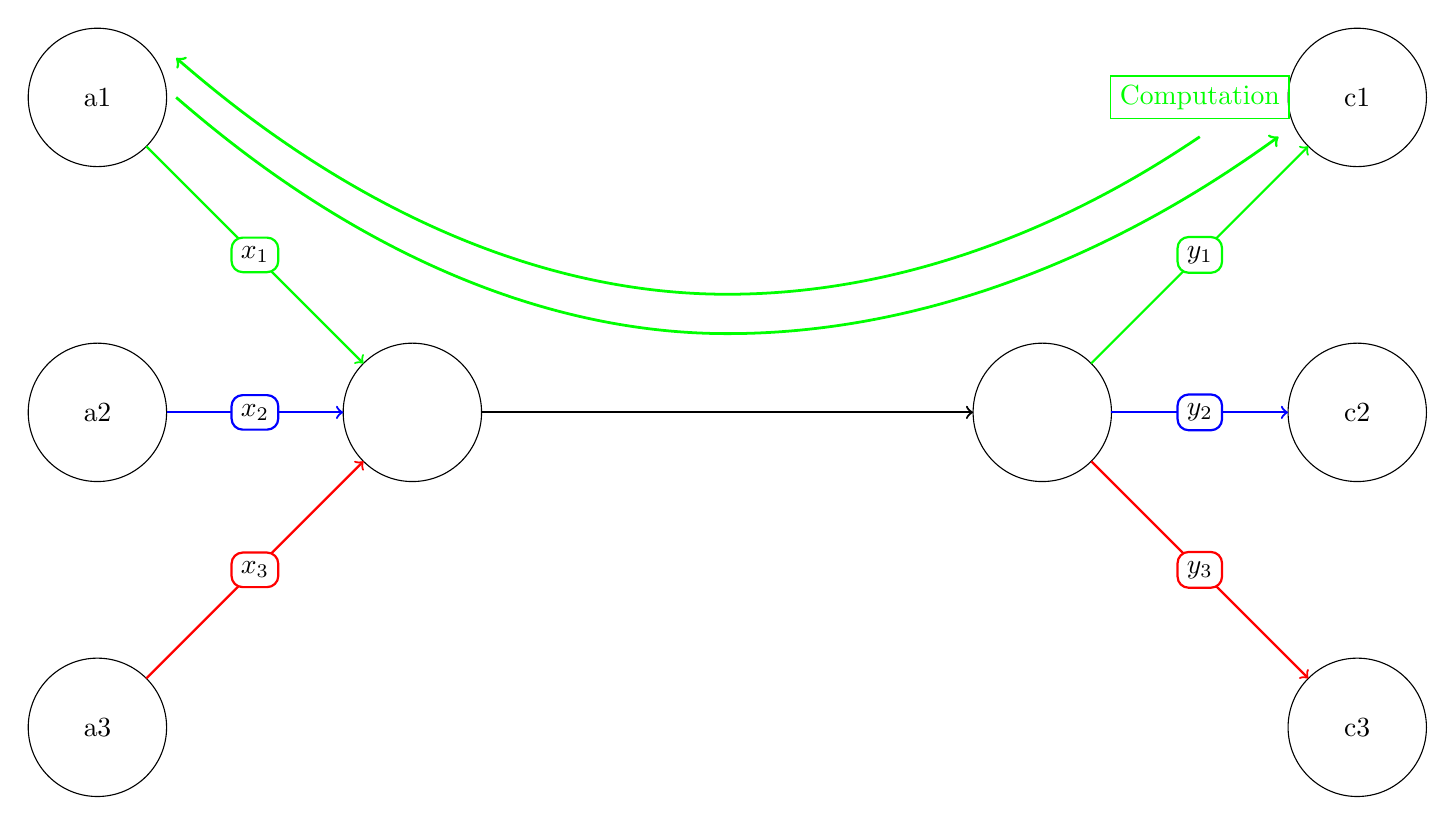
\begin{tikzpicture}
    \SetGraphUnit{5}
  \tikzstyle{VertexStyle}=[shape = circle, draw, minimum size = 50pt]
  \Vertex[x=0,y=0]{a3}
  \Vertex[x=0,y=4]{a2}
  \Vertex[x=0,y=8]{a1}
  
  \Vertex[x=16,y=0]{c3}
  \Vertex[x=16,y=4]{c2}
  \Vertex[x=16,y=8]{c1}
  
  \SetVertexNoLabel
  \Vertex[x=4,y=4]{SL}
  \Vertex[x=12,y=4]{SS}  
  \tikzset{
  EdgeStyle/.append style = {<-,green} }
  \Edge[label = $y_1$](c1)(SS)
  \Edge[label = $x_1$](SL)(a1)
  
  \tikzset{
  EdgeStyle/.append style = {blue} }
  \Edge[label = $y_2$](c2)(SS)
  \Edge[label = $x_2$](SL)(a2)
  
  \tikzset{
  EdgeStyle/.append style = {red} }
  \Edge[label = $y_3$](c3)(SS)
  \Edge[label = $x_3$](SL)(a3)
  
  \tikzset{
  EdgeStyle/.append style = {black} }
  \Edge(SS)(SL)
  
  \draw[->,line width=1pt,green] (1,8) parabola bend (8,5) (15,7.5);
  \node[draw,green] at (14,8) {Computation};
  \draw[<-,line width=1pt,green] (1,8.5) parabola bend (8,5.5) (14,7.5);


\end{tikzpicture}
}

The second scheduling depends of the first.

The goal is to minimise the maximal latency on the routes.

\end{frame}

\end{section}


\begin{frame}{Longest Shortest Greedy versus Random}
   \centering
    \begin{tabular}{c c}
     % \includegraphics[scale=0.2]{distriscumul_longest.pdf} &  \includegraphics[scale=0.2]{distriscumul_random.pdf}\\
      LSG & Random \\
    \end{tabular}
     LSG $\rightarrow$ far from the deadline.
     
    Random $\rightarrow 10\%$ solutions with $T_{max} >$ deadline for 5 flows.

\end{frame}

\end{section}

\begin{section}{Conclusion}
 

\begin{frame}{Conclusion}

\underline{\bf{\large Results:}}
\begin{itemize}
 \item An heuristic giving good results compared to statistical approach.
 \item An Algorithm giving optimal solutions for some parameters. 
\end{itemize}
\vspace{1cm}
\underline{\bf{\large Further research:}}
\begin{itemize}
 \item Improve the model.
 \item Study other topologies.
\end{itemize}



\end{frame}

\end{section}


\end{document}
